\documentclass[a0,portrait]{a0poster}
\usepackage{graphicx}
\usepackage{multicol}
\usepackage{charter}
\usepackage{color}
\usepackage[utf8]{inputenc}
\usepackage{amsmath}
\usepackage{caption}
\usepackage{enumitem}
\usepackage{booktabs}
\usepackage{xcolor}
\usepackage{array}
\usepackage{parskip}          % Activa el paquete para controlar el espacio entre párrafos
\usepackage{comment} %sirve para agregar comentarios en mas de una línea del código
% Incluir el paquete tcolorbox para crear cuadros de colores
\usepackage{tcolorbox}

\renewcommand{\figurename}{Gráfico}
\definecolor{miRojo}{rgb}{0.82, 0.32, 0.31}  % Definir el color usando valores rgb
\definecolor{lightgray}{gray}{0.9}  % Color gris claro para subrayado
\definecolor{miGray}{gray}{.6}  % Color gris claro para subrayado
\definecolor{miVerde}{rgb}{0.0, 0.6, 0.0}  % Definir un color verde personalizado
\setlength{\parindent}{2em}   % Ajusta la sangría global
\setlength{\parskip}{2em}     % Ajusta el espacio entre párrafos

\setlength{\columnsep}{2cm}
\setlength{\columnseprule}{2.5pt}
\def\columnseprulecolor{\color{miRojo}}


% Crear comando para secciones subrayadas y centradas con cuadro azul
\newcommand{\customsection}[1]{
    \begin{center}
        \begin{tcolorbox}[colframe=miRojo!50, colback=miRojo, width=\linewidth, boxrule=1mm, arc=3mm, auto outer arc]
            \centering
            \vspace{.5cm} % Espacio entre el parrafo anterior y el subtitulo
            \color{white}
            \textbf{\Huge #1}
            \color{miRojo}
            %\vspace{.5cm} % Espacio entre el título y la línea
            %\hrule height 2.5pt  % Línea subrayada gris
            \vspace{.5cm} % Espacio después de la línea
        \end{tcolorbox}
    \end{center}
}

\begin{document}
% Recuadro inicial en todo el ancho de la hoja sin márgenes
\begin{tcolorbox}[colframe=miGray, colback=miGray!40, width=\linewidth, boxrule=1mm, arc=3mm, left=0pt, right=0pt, top=0pt, 
    bottom=0pt, boxsep=0pt]
    \centering
        
\includegraphics[width=.3\linewidth]{logo_fae_web.png}\\
        \vspace{-2.5cm} % Ajusta este valor si es necesario para el espaciado
        \VeryHuge \textbf{\emph{Evaluación del poder predictivo de estrategias técnicas de tendencia y momentum sobre acciones 
        americanas}}\par
        \vspace{1cm}
        \Huge Mateo Canales Briceño, Cristóbal González Araya, Tomás Leyton Muñoz \par
        \LARGE Escuela de Ingeniería Comercial, Universidad Diego Portales, 2024 \par
        \vspace{1cm}

\end{tcolorbox}

\vspace{2cm}
\normalsize %tamaño de la letra, recomiendo Large
\begin{multicols}{2}

    % Sección 1: Resumen
    \customsection{Resumen}
    \par
    \normalsize
    Esta tesis evalúa el poder predictivo de estrategias técnicas de tendencia y momentum sobre el mercado de acciones americanas.
     Utilizando indicadores técnicos, se implementaron modelos econométricos para predecir la dirección de las acciones en el 
     índice \textit{S\&P500} y evaluar su significancia. Los resultados sugieren que al menos la mitad de los indicadores son significativos, lo que valida el uso 
     de estas estrategias en la toma de decisiones de inversión.
    
    % Sección 2: Introducción
    \customsection{Introducción}
    \par
     En las últimas décadas, el mercado de acciones de EE. UU. ha experimentado cambios significativos, lo que ha llevado al
      desarrollo de estrategias técnicas como tendencia y momentum. Estas estrategias, basadas en análisis de datos históricos, 
      son herramientas clave para predecir movimientos futuros en los precios de las acciones.
    % Sección 3: Metodología
    \customsection{Datos}
    \par
    %betas añadir
    Se utilizó una base de datos que abarca desde enero de 2019 hasta julio de 2024, con periodicidad de precios de cierre 
    diarios obtenidos de Yahoo Finance.\\
    % Tabla con minipage
    \begin{minipage}{,984\linewidth}
        \centering
        \vspace{1cm}
        \captionof{table}{Disección por \textit{Betas}.}
        \begin{tabular}{cc}
            \toprule
            \textbf{Grupo} & \textbf{\textit{Beta}}  \\
            \midrule
            1   &  $\beta < 0.5$                      \\
            2       & $0.5 \leq \beta \leq 1$    \\
            3      & $1 < \beta \leq 1.5$    \\
            4       & $1.5 < \beta $    \\
            5       & $\beta =N/A$    \\
            \bottomrule
            \vspace{.5cm}
        \end{tabular}
        \end{minipage}
    \customsection{Metodología}
    \par
    \textbf{Datos:} Se utilizó una base de datos que abarca desde enero de 2019 hasta julio de 2024, con periodicidad de precios
     de cierre diarios obtenidos de Yahoo Finance. Además, se subdividieron los datos en 5 grupos según el \textit{Beta} asociado al ticker.  
    \par
    \textbf{Indicadores técnicos:} Apartir de los indicadores técnicos se generan señales de compra (1) y venta (0) asumiendo que si el período anterior
     los que posteriormente generan señales binarias de 0 y 1.\\
     \begin{minipage}{,984\linewidth}
        \centering
        \vspace{1cm}
        \captionof{table}{Lista de indicadores técnicos.}
        \begin{tabular}{ccl}
            \toprule
            \textbf{Indicador Técnico} & \textbf{Parámetros} & \textbf{Descripción}\\
            \midrule
             SMA & (1,50), (1,150), (1,200), (5,200)  & (Medias Móviles Simples)\\
             MACD & (12,26,9) & (Convergencia/Divergencia) \\
             ROC & (10), (50), (200) & (Tasa de Cambio) \\
             RSI & (14), (20), (50) & (Índice de Fuerza Relativa) \\
             WLPR & (14), (20), (50) &  (Williams \%R)\\
            \bottomrule
        \end{tabular}
        \captionsetup{width=0.8\textwidth}  % Ajusta el ancho del pie de tabla
        \caption*{\footnotesize Donde $SMA(x,y)$ $x$ corresponde a la ventana de tiempo corta, $y$ correspponde a la ventana de tiempo larga.}
        \end{minipage}
    \par
    \textbf{Modelos Econométricos:} Se construyeron varios modelos de regresión lineal para evaluar la capacidad predictiva de 
    estos indicadores técnicos. Las regresiones se estimaron con HAC según Newey-West (1987). Las señales tecnicas se construyen 
    a base de los precios, arrojando 0 cuando la ventana corta es menor que la larga y 1 cuando es mayor. Tras obtener estas 
    variables dummy, se construyen las regresiones y se analiza la significancia de 
    las señales. 
    
    La ecuación general del modelo de regresión utilizado es la siguiente:

\begin{minipage}{.984\linewidth}
    \centering
    \vspace{1cm}
    \captionof{table}{Modelos de Regresión Utilizados.}
    \begin{tabular}{cl}
        \toprule

        \textbf{Modelo} & \multicolumn{1}{c}{\textbf{\textit{Regresión}}}   \\
        \midrule
        (1) & $R_t = \alpha +\beta_1 \cdot R_{t-1} + \beta_2 \cdot Signal_{j,t-1} + \varepsilon_t$ \\
        (2) & $R_t = \alpha +\beta_1 \cdot R_{t-1} + \beta_2 \cdot Signal_{j,t-1} + \beta_3 \cdot Signal_{j,t-2}+ \varepsilon_t$ \\
        (3) & $R_t = \alpha +\beta_1 \cdot R_{t-1} + \beta_2 \cdot Signal_{j,t-1} + \beta_3 \cdot Signal_{j,t-2}+\beta_4 \cdot Signal_{j,t-3}+\varepsilon_t$ \\
        \bottomrule
    \end{tabular}
    \captionsetup{width=0.8\textwidth}  % Ajusta el ancho del pie de tabla
    \caption*{\footnotesize Donde: $R_t$ es el retorno en el tiempo $t$, $\text{SIGAL}$ es una variable dummy \{0,1\}, $j$ es 
    el indicador técnico,     $\alpha$ es la interseccion, $\beta_1$, $\beta_2$, y $\beta_3$ son los coeficientes estimados.
    $\varepsilon_t$ es el término de error en el tiempo $t$.    }  % Pie de tabla
    \vspace{.5cm}
    \end{minipage}
       
                
                
\columnbreak
    % Sección 4:Resultados
    \customsection{Resultados}
    \par 
     \normalsize
     Para poder presentar los datos de manera mas ordenada, los tickers se divideron según el \textit{Beta} que se obtiene
      desde yahoo finance, dónde el grupo\\
    Como resultado de las regresiones de los 504 tickets, la base fue diseccionada tomando solo aquellas empresas 
    que han tenido un crecimiento constante durante los ultimos 5 años, ya que sus retornos reflejan esta informacion, 
    haciendo que nuesto modelo fuera de muestra presente mayor significancia y probabilidades de predecir con exito el 
    retorno de estas acciones.
    

    \vspace{1cm}
    \begin{comment}
        
        % Tabla con minipage
        \begin{minipage}{,984\linewidth}
        \centering
        \captionof{table}{Resultados de los coeficientes para diferentes benchmarks.}
        \begin{tabular}{ccccccc}
        \toprule
        \textbf{Grupo} & \textbf{pollo} & \textbf{Leyton} & \textbf{Por-ano} & \textbf{Sacamos oro} & \textbf{detroit} \\
        \midrule
        1   & 1.217*  & 3.684*** & 2.45** & 0.074  & 1.473*  \\
        2       & 1.535*  & 2.927**  & 2.379* & 0.149  & 1.586** \\
        3       & 1.52*   & 2.903**  & 2.374* & 0.144  & 1.579*  \\
        4       & 1.213*  & 3.576**  & 2.344* & 0.1427 & 1.625** \\
        5    & 1.131*  & 3.824*** & 2.489** & 0.028  & 1.456** \\
        \bottomrule
        \vspace{.5cm}
    \end{tabular}
\end{minipage}
\end{comment}
    % Gráfico con minipage  
    \begin{minipage}{\linewidth}
    \centering
    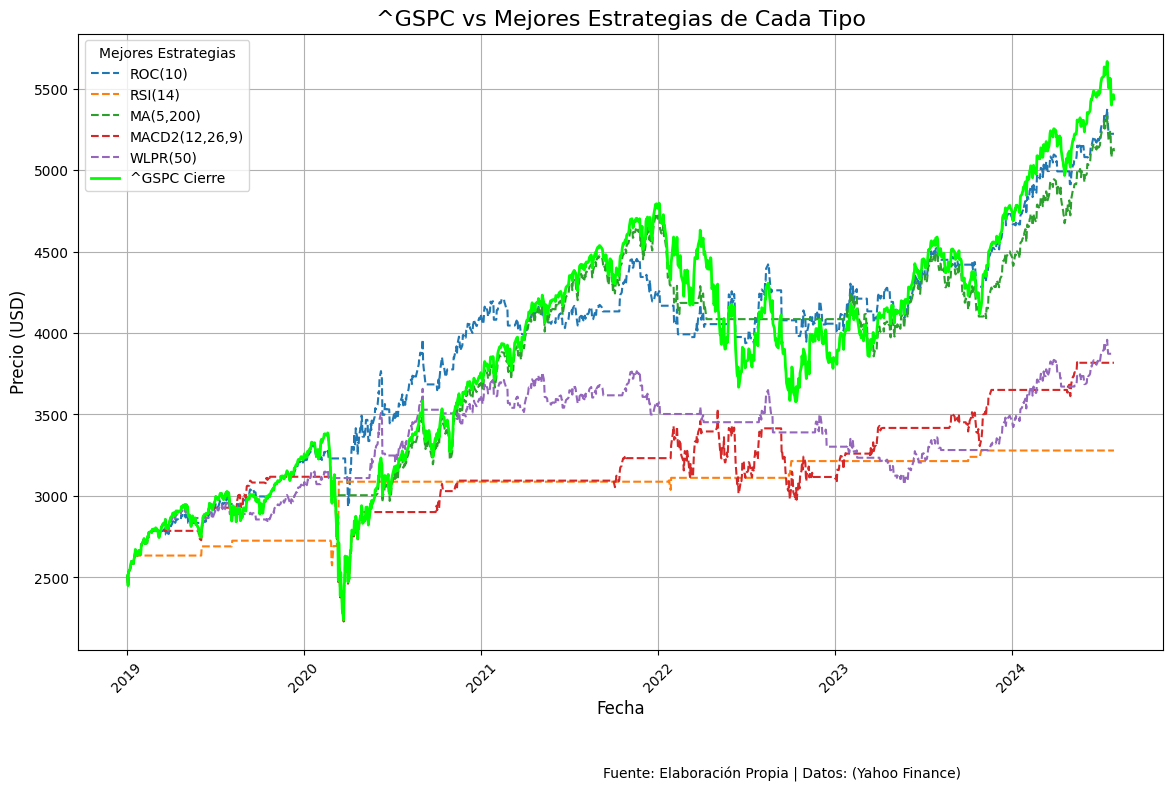
\includegraphics[width=0.9\linewidth]{grafico_mejores_estrategias_^GSPC.png}
    
    \captionof{figure}{Este grafico representa las mejores estrategias de cada tipo de indicador, y es aplicado al ticker 
    \emph{\textasciicircum GSPC} correspondiente al índice \textit{S\&P500}.}
    \end{minipage}
    % Sección 5: Conclusiones
    \customsection{Conclusiones}
    \par
    \indent La investigación valida el uso de estrategias de tendencia y momentum para predecir el mercado de acciones 
    estadounidense. Estas herramientas son valiosas para los inversores que buscan optimizar su toma de decisiones en un 
    entorno bursátil dinámico. 
    % Sección 6: Referencias   
    \customsection{Referencias}
    \par
         \begin{itemize}
            \item Gradojevic (2023) Forecasting Bitcoin with technical analysis: A not-so-random forest?
            \item Ifleh et al. (2023). Stock price indices prediction combining deep learning algorithms and selected technical 
            indicators based on correlation
            \item Jegadeesh, N., y Titman, S. (1993). Returns to buying winners and selling losers: Implications for stock 
            market efficiency.
            \item Lim, B. Y., Wang, J. G., y Yao, Y. (2018). Time-Series Momentum in nearly 100 years of stock returns.            
            \item Subrahmanyam, A. (2018). Equity market momentum: A synthesis of the literature and suggestions for future work.
            \item Wu et al. (2020) Adaptive stock trading strategies with deep reinforcement learning methods
        \end{itemize}
        
    
    
    
    
\end{multicols}
\end{document}
